\subsection{Tabs toevoegen}\label{tabstoevoegen}
Aan alle inhoudstypen kunnen "Tabs" toegevoegd worden. 
Tabs toevoegen kan alleen bij velden waarbij de WYSIWYG editor geactiveerd is; op het veld "Body" is vrijwel altijd de WYSIWYG editor geactiveerd.

Een tab moet opgebouwd worden uit twee delen: de titel van de tab en de content van de tab.

\textbf{Een tab toevoegen:} 

\begin{enumerate}
\item Vul twee asterisken in (**), gevold door een spatie en vul vervolgens de titel van de tab in (** Tab1).
\item Selecteer met je muis de hele regel (zie screenshot).
\item Maak van deze selectie een \emph{H2} (heading 2).
\item Druk op de enter toets om naar de volgende regel toe te gaan, vul hier de inhoud van de tab in.
\item Herhaal deze stappen indien je meerdere tabs wil toevoegen.
\end{enumerate}

De onderstaande screenshot toont visueel aan hoe je tabs kunt toevoegen.

\begin{center}
	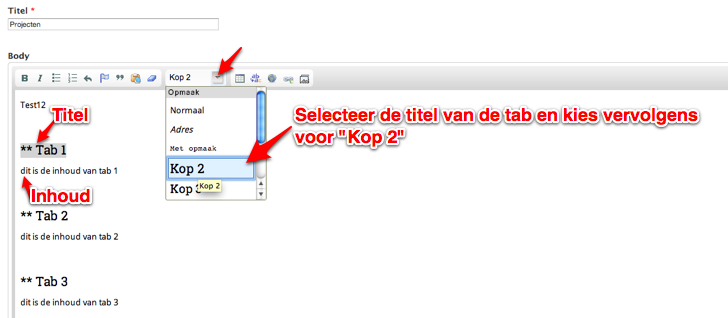
\includegraphics[width=\textwidth]{img/tabs1}
\end{center}

De onderstaande screenshot toont het resultaat.

\begin{center}
	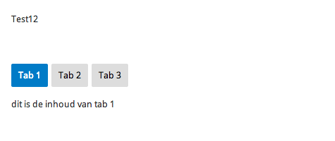
\includegraphics[width=\textwidth]{img/tabs2}
\end{center}